\RequirePackage{luatex85}
\documentclass[a4paper,sfsidenotes,twoside,justified]{tufte-book-custom}
% \usepackage{showframe}

\hypersetup{colorlinks}

\title[On Homomorphism Problems]{ Homomorphism\\ Problems: from Minimization of Graph Databases Queries to the Frontier of Decidability in Automatic Structures}
\author[The Tufte-LaTeX Developers]{The Tufte-LaTeX\ Developers}
\publisher{Publisher of This Book}

\usepackage{microtype}
\usepackage{booktabs}
\usepackage{graphicx}
\usepackage{lipsum}

\newrobustcmd{\fancyand}{{\setmainfont{Tex Gyre Pagella}\textit{\&}}}
\setcounter{secnumdepth}{3}

% https://coolors.co/001219-005f73-0a9396-94d2bd-e9d8a6-ee9b00-ca6702-bb3e03-ae2012-9b2226

\usepackage[UKenglish]{babel}
\usepackage{xcolor}

\definecolor{Rich Black}{HTML}{001219}
\definecolor{Blue Sapphire}{HTML}{005f73}
\definecolor{Viridian Green}{HTML}{0a9396}
\definecolor{Middle Blue Green}{HTML}{94d2bd}
\definecolor{Medium Champagne}{HTML}{e9d8a6}
\definecolor{Gamboge}{HTML}{ee9b00}
\definecolor{Alloy Orange}{HTML}{ca6702}
\definecolor{Mahogany}{HTML}{bb3e03}
\definecolor{Rufous}{HTML}{ae2012}
\definecolor{Ruby Red}{HTML}{9b2226}

\definecolor{Dark Red}{HTML}{9d0208}
\colorlet{maincolor}{Ruby Red}

\RequirePackage{amsmath}
\RequirePackage{amssymb}
\RequirePackage{latexsym}
\RequirePackage{mathtools}
\RequirePackage{fontenc}
\RequirePackage{unicode-math}
\setmainfont{Libertinus Serif}
\setsansfont{Libertinus Sans}
\setmonofont[Scale=0.8]{Libertinus Mono}
\setmathfont[math-style=TeX]{Asana Math}
\setmathfont[math-style=TeX, range={cal, bfcal}]{Latin Modern Math}

\begin{document}

\frontmatter
\newgeometry{hmargin=2.5cm, top=4.5cm, bottom=3cm}
\begin{titlepage}
\begin{center}
  \Huge\scshape%
  Homomorphism Problems
  \LARGE\\
  in Graph Databases\\
  and Automatic Structures\\
  % \vspace{5cm}
  % \makebox[0pt]{{%
  %   \fontsize{50}{0}\selectfont\color{black!11}%
  %   $\gamma \equiv^{?} \delta$%
  % }}{}\\
  \vfill
  \normalfont\LARGE{} \textsc{Rémi Morvan}\\[1em]
  \Large\scshape
  Ph.D. thesis in Computer Science\\
  \textcolor{maincolor}{LaBRI, Université de Bordeaux}\\
  \normalfont\Large\scshape To be defended on 3rd July 2025
\end{center}
\end{titlepage}
\restoregeometry
\newpage
\thispagestyle{empty}
~
\newpage
\thispagestyle{empty}
% \setlength{\parskip}{\baselineskip}
\begin{fullwidth}
	\setlength{\parindent}{0pt}
	~\vfill
	\begin{center}
		\normalfont\Large\scshape Composition of the jury:\\[1.5em]
		\normalfont
		\begin{tabular}{r@{\hskip 1em}l@{\hskip 1em}l}
		  Mikołaj Bojańczyk & \textsc{\small Uniwersytet Warszawski} & \emph{reviewer {\small\fancyand}~examiner}\\
		  Wim Martens & \textsc{\small Universität Bayreuth} & \emph{\hphantom{revi}``} \\[.5em]
		  Antoine Amarilli & \textsc{\small Inria, Lille} & \emph{examiner}\\
		  Balder ten Cate & \textsc{\small Universiteit van Amsterdam} & \emph{\hphantom{revi}``}\\
		  Bartek Klin & \textsc{\small University of Oxford} & \emph{\hphantom{revi}``}\\
		  Anca Muscholl & \textsc{\small Université de Bordeaux} & \emph{\hphantom{revi}``}\\
		  Sophie Tison & \textsc{\small Université de Lille} & \emph{\hphantom{revi}``}\\[.5em]
		  Diego Figueira & \textsc{\small CNRS, Bordeaux} & \emph{supervisor}\\
		  Nathanaël Fijalkow & \textsc{\small CNRS, Bordeaux} & \emph{co-supervisor}
		  % Sophie Tisson
		\end{tabular}
	\end{center}

	\vfill

	\par\textsc{Licensed under "CC BY 4.0".}
	\par\textit{Version of \today.}
\end{fullwidth}
% r.5 contents
{ % env necessary for the parskip not to leak in the rest of the doc.
	\setlength{\parskip}{0em}
	% \addcontentsline{toc}{chapter}{Contents}
	\setcounter{tocdepth}{1}
	\tableofcontents
}
% \listoffigures
% \listoftables

% % r.7 dedication
% \cleardoublepage
% ~\vfill
% \begin{doublespace}
% \noindent\fontsize{18}{22}\selectfont\itshape
% \nohyphenation
% Dedicated to those who appreciate \LaTeX{} 
% and the work of \mbox{Edward R.~Tufte} 
% and \mbox{Donald E.~Knuth}.
% \end{doublespace}
% \vfill
% \vfill


\mainmatter
\chapter{Ideas/Todos}

\begin{itemize}
	\item Change definition of CQ/CRPQ to have vertices. This allows for better duality,
		and also better statement for the Semantical Structure Theorem (in some prop we get
		``foo is an edge cotnraction of bla'' instead of ``is a minor of'').
		Update the definition of `one-way internal path' to allow for $n=0$.
	\item Extend the notion of `strong minimality` using the axioms used in the lower bound (`str-onto`): call such canonical databases / extensions `structurally minimal'.
	Prove or disprove the following result: ``a "CRPQ" has "one-way semantic tree-width" at least $k$ "iff" it has an expansion that is structurally minimal and whose core has tree-width at least $k$''. In general: what about minor-closed classes?
	Extend Grohe's Theorem to CRPQs (or maybe to a subclass of CRPQs, "eg" those whose
	structurally minimal canonical databases characterize membership to minor-closed classes).
\end{itemize}

\chapter{Introduction}

\part{Querying Graph Databases}

\chapter{Preliminaries on Graph Databases}

\section{Elementary Notations}

\subsection{Blabla}

% \begin{figure}
% 	\centering
% 	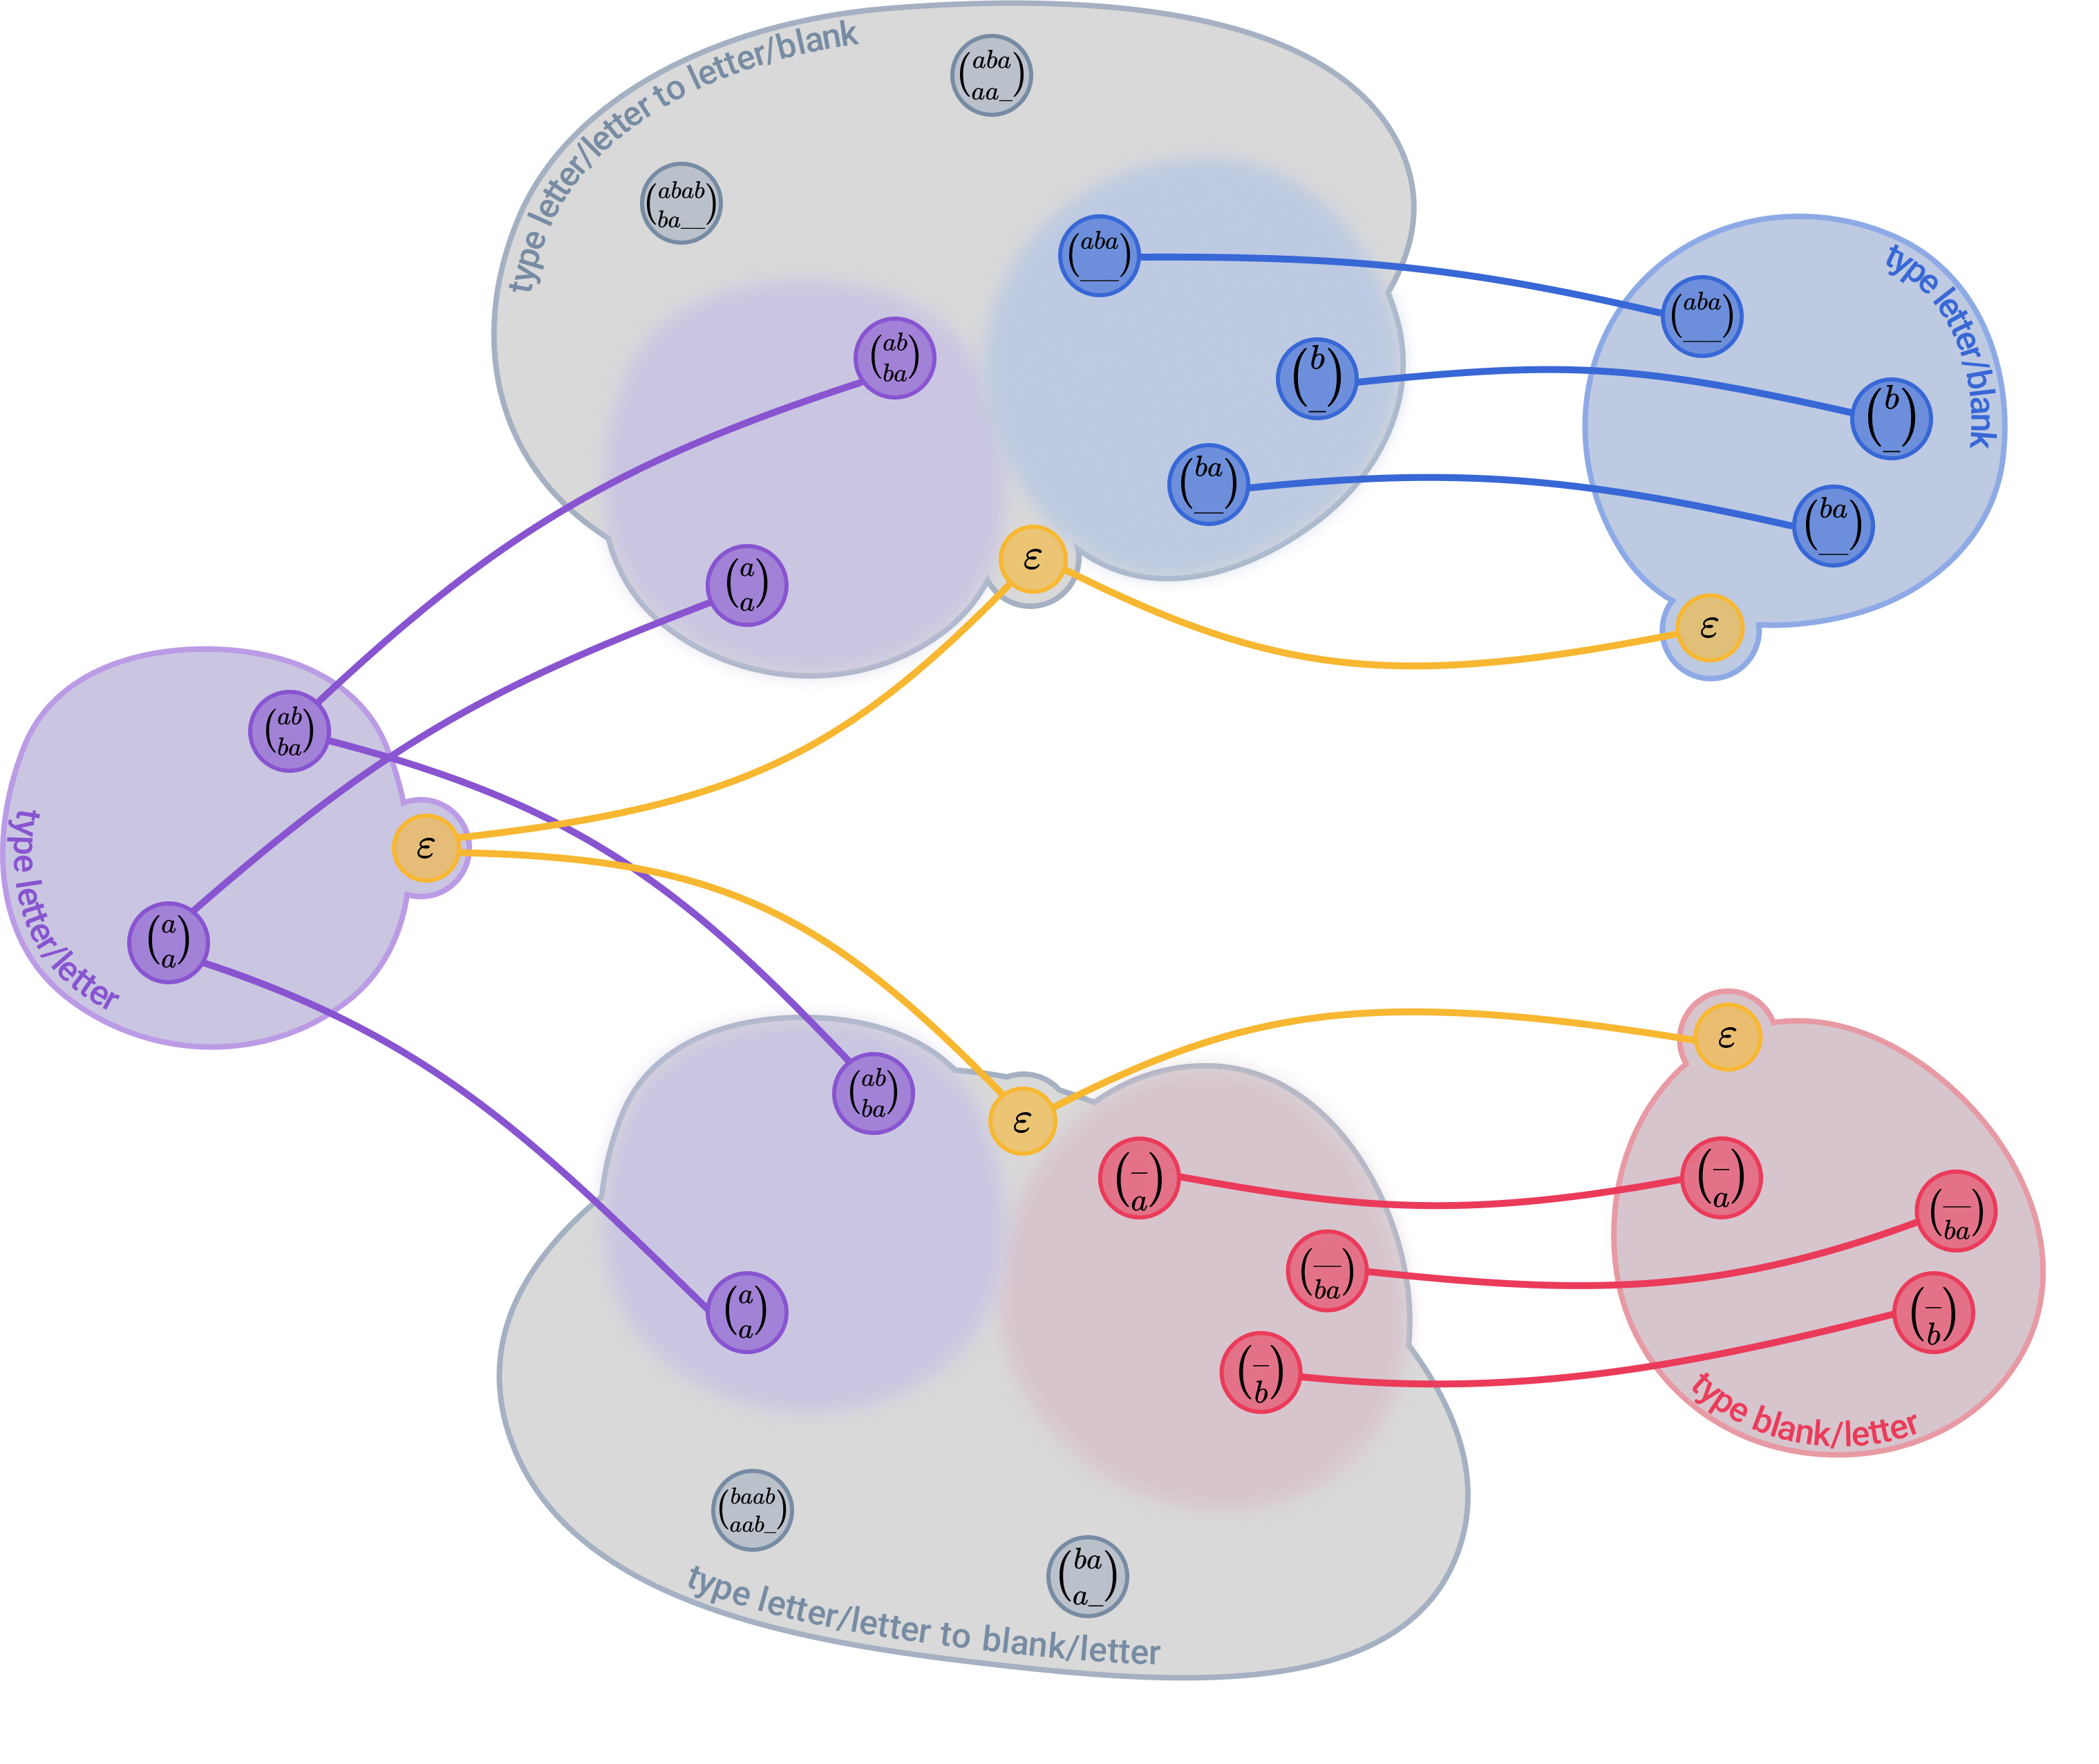
\includegraphics[width=\linewidth]{fig/free_algebras.png}
% 	\caption{My super nice caption.}
% \end{figure}

\begin{table}
	\centering
	\begin{tabular}{cc}
		\toprule
		a & b \\ \midrule
		0 & 1 \\
		1 & 0 \\ \bottomrule
	\end{tabular}
	\caption{My super nice caption.}
\end{table}

Hello this is a citation\cite{Bringhurst2005}.
Hello Q\sidenote{Qy first sidenote!} world\sidenote{Another side note}.
\[\forall x \in \gamma,\, \exists y\in \delta, \delta \to \gamma\]
\[L \subseteq \Sigma^*\]
\[0 \in \mathbb{N}\]
\[\mathcal{AbcDefGhiJkl}\]

\lipsum[1-2]

\begin{figure}[htb]
	\centering
	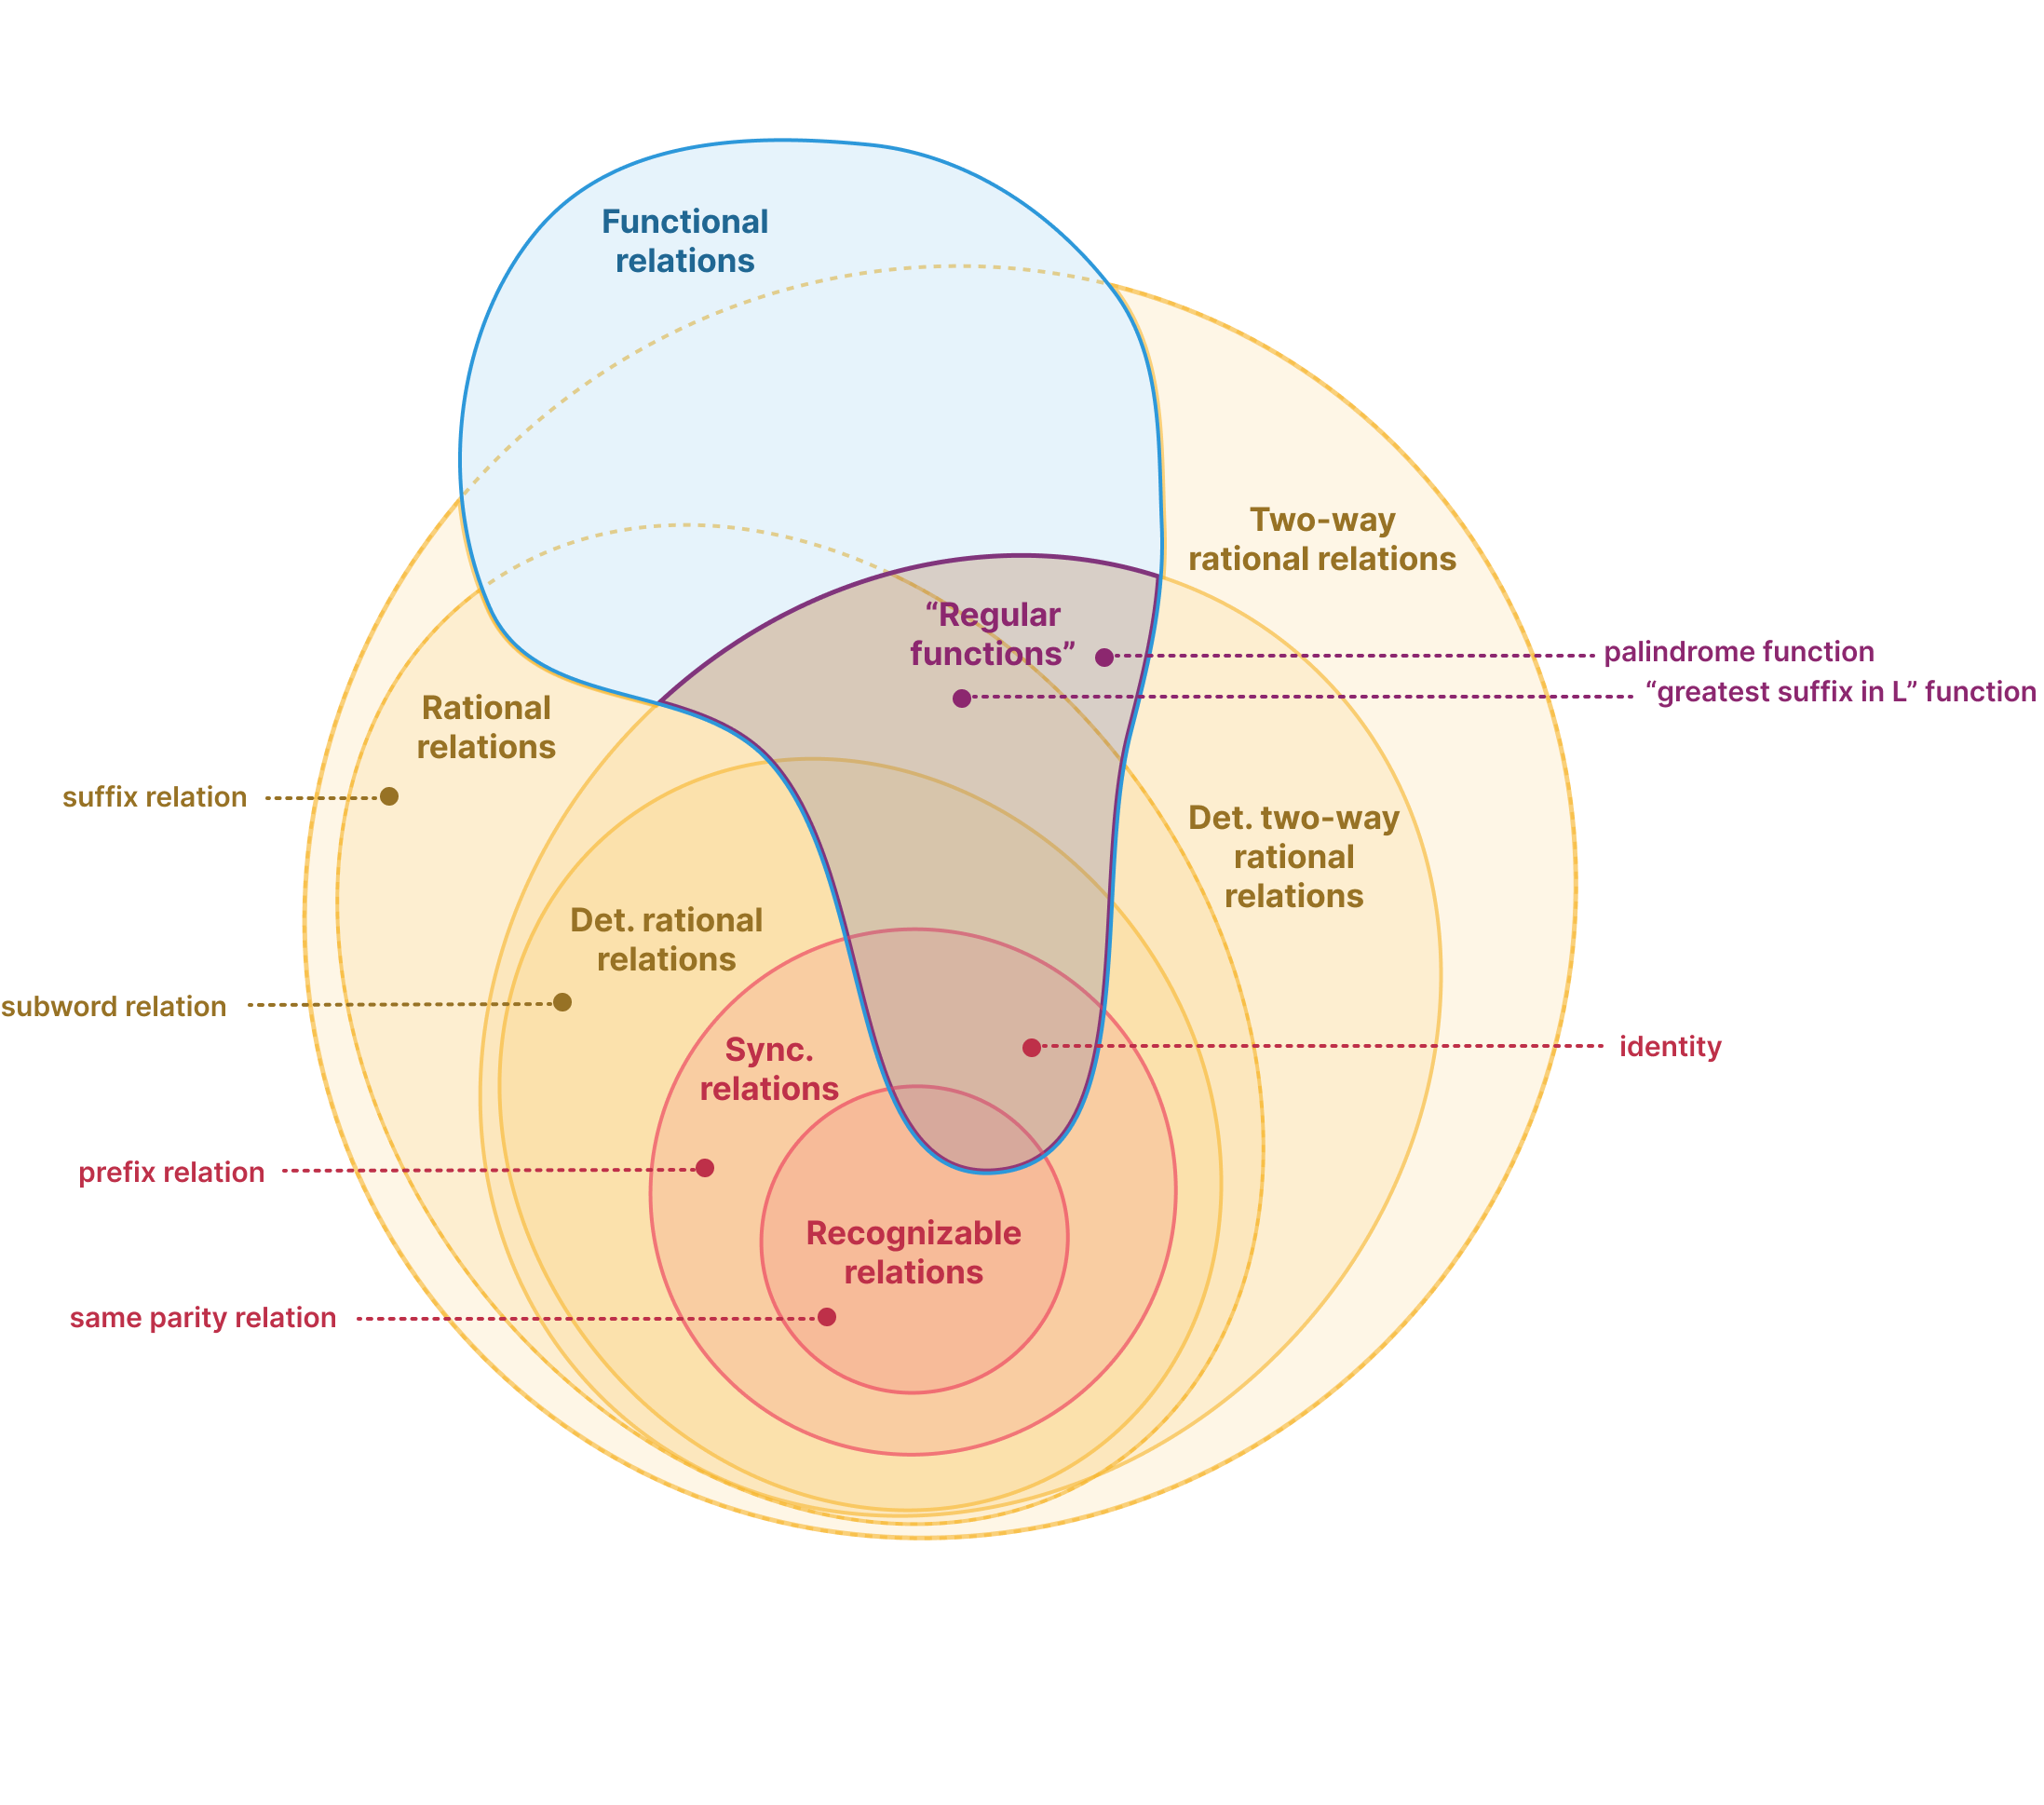
\includegraphics[width=\linewidth]{fig/landscape.png}
	\caption{The landscape of rationality.}
\end{figure}

\lipsum[3-10]

\chapter[Evaluation and Containment of Conjunctive Regular Path Queries]{Evaluation and Containment\\ of Conjunctive Regular Path Queries}

\chapter{Minimization of Conjunctive Regular Path Queries}

\chapter[{Semantic Tree-Width and Path-Width of Conjunctive Regular Path Queries}]{Semantic Tree-Width and Path-Width\\of Conjunctive Regular Path Queries}

\chapter{Synthesis of Conjunctive Regular Path Queries}

\chapter{Conclusion \& Open Problems}

\part[The Frontier of Decidability in Automatic Structures]{The Frontier of Decidability\\in Automatic Structures}

\chapter{Preliminaries on Automatic Structures}

\chapter{A Dichotomy Theorem for Automatic Structures}

\chapter{The Algebras for Automatic Relations and Beyond:\\the Relative Membership Problem for Pseudovarieties of Regular Languages}

\chapter{Conclusion \fancyand~Open Problems}


\backmatter

\bibliography{sample-handout}
\bibliographystyle{plainnat}

\end{document}

